\chapter{Numerical Integration}\label{chapter:numerical_integraion}
\section{Numerical Integration - Trapezoidal rule}
\index{Trapezoidal rule}
\index{Weights}
In this chapter, we will briefly review the concepts of numerical integration in one dimension. Consider an integral over some function $f(\omega)$
\begin{equation}
	I=\int_a^b d\omega f(\omega)
\end{equation}
For the numerical calculation of this integral one has to discretize the interval of integration $[a,b]$:
\[
	\omega(i) \quad;\quad i\in\{0,\dots,M\}\quad\text{and}\quad \omega(0)=a,\quad \omega(M)=b.
\]
Where the strictly increasing mapping $\omega: \mathbbm{N} \to \mathbbm{R}: i \mapsto \omega(i)$ is called a grid. The numerical approximation for the integral now reads
\begin{equation} 
	I=\sum_{i=0}^M d\omega(i) f(\omega(i))
\end{equation}
where the $d\omega(i)$ are the so-called weights. There are various methods to calculate the weights out of the grid itself. We will restrict ourselves to the trapezoidal rule which approximates the integrand function by linear regions connecting the sample points (see figure~\ref{fig:trapezoidal_rule}).
\begin{figure}[ht]
	\centering
	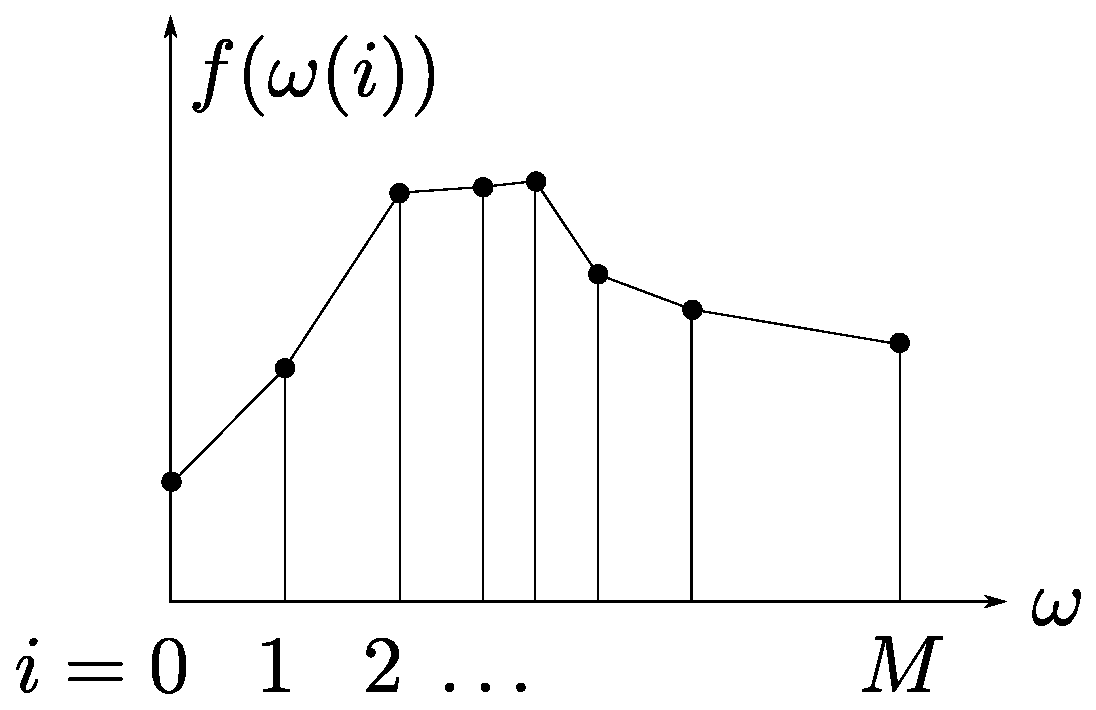
\includegraphics[width=0.3\textwidth]{pics/trapez.eps}
	\caption{Trapezoidal rule for a non-equidistant grid.}
	\label{fig:trapezoidal_rule}
\end{figure}

The numerical approximation for the integral is then
\begin{align*}
	I&=\sum_{i=0}^{M-1} \frac{f(\omega(i+1)) + f(\omega(i))}{2} (\omega(i+1)-\omega(i)) \\
	&=f(a)\biggl( \underbrace{\frac{\omega(1)-\omega(0)}{2}}_{d\omega(0)}\biggr) + f(b) \biggl( \underbrace{\frac{\omega(N)-\omega(N-1)}{2}}_{d\omega(N)}\biggr) + \sum_{i=1}^{M-1} f(\omega(i)) \biggl( \underbrace{\frac{\omega(i+1)-\omega(i-1)}{2}}_{d\omega(i)}\biggr)\\
	&=\sum_{i=0}^{M} d\omega(i)\,f(\omega(i)).
\end{align*}
Therefore the weights are given by
\[
	d\omega(i)=\begin{cases}
		\frac{\omega(1)-\omega(0)}{2} \quad &i=0\\
		\frac{\omega(i+1)-\omega(i-1)}{2} \quad &i\in \{1,\dots,M-1\}  \\
		\frac{\omega(N)-\omega(N-1)}{2} \quad &i=\,.
	\end{cases}
\]

\section{Interpolation - Inverse mapping}\index{Interpolation}
\index{Inverse mapping}
In order to calculate a function $f$ which is known on a given grid $\omega(i)$, on another grid $\epsilon(i)$ one needs to interpolate. We restrict ourselves to linear interpolation and we further assume, that the inverse mapping of the first grid
\[
	i(\omega):\;\mathbbm{R}\to\mathbbm{N}:\quad \omega \mapsto i\quad\quad;\;\omega\in[\omega(0), \omega(M)]
\]
is known.

The interpolation is then done in the following way. For each point of the new grid $\epsilon(j)\equiv \epsilon_j$ one calculates the inverse of the old grid $I=i(\epsilon_j)$. The corresponding old grid point $\omega(I)\equiv \omega_I$ is then the nearest grid point to the interpolation point $\epsilon_j$ (Figure~\ref{fig:interpolation}). 
\begin{figure}[ht]
	\centering
	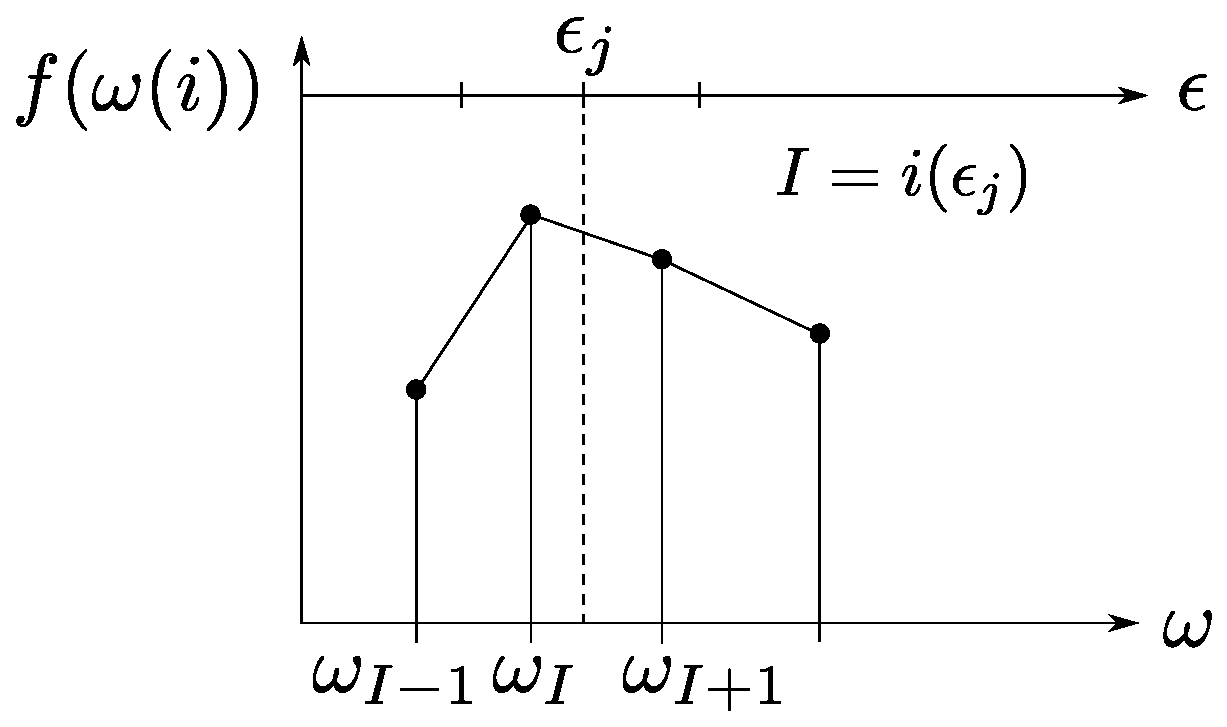
\includegraphics[width=0.4\textwidth]{pics/interpolation.eps}
	\caption{Linear interpolation of $f(\{\omega_i\})$ on a new grid $\{ \epsilon_j \}$}
	\label{fig:interpolation}
\end{figure}

The value of the function on a point $\epsilon_j$ of the new grid $f(\epsilon_j)$ is then obtained by linear interpolation between the old grid point $\omega_I$ and its nearest neighbor (right neighbor for $\omega_I\leq\epsilon_j$, left neighbor for $\omega_I>\epsilon_j$).
\[
	f(\epsilon_j)=\begin{cases}
		f(\omega_I)+\frac{f(\omega_{I+1})-f(\omega_{I})}{\omega_{I+1}-\omega_{I}} (\epsilon_j-\omega_I) \quad \text{for } \omega_I<\epsilon_j \\
		f(\omega_I)+\frac{f(\omega_{I-1})-f(\omega_{I})}{\omega_{I-1}-\omega_{I}} (\epsilon_j-\omega_I) \quad \text{for } \omega_I>\epsilon_j 
	\end{cases}
\]






